\documentclass[a4paper, titlepage]{article} % defines Basic settings for my document

\usepackage[german]{babel} %Imports Package for german Language Support
\usepackage{blindtext} %Imports Package for creating Blindtext
\usepackage{booktabs, bookmark}
\usepackage{tabularx}
\usepackage{microtype} %Imports Package for ...
\usepackage{graphicx} %Imports Package for using Graphics
\usepackage{wrapfig} %Imports Package for Wrap Text around Graphics
\usepackage{enumitem} %Package for nicer looking lists
\usepackage{fancyhdr} %Nicer Header
\usepackage{amsmath} %formulas
\usepackage{index} %for Indexes
\usepackage{caption, subcaption}
\usepackage{chngcntr}
\usepackage{listings}
\usepackage{xcolor}
\usepackage{hyperref}
\usepackage{color}

\usepackage[a4paper, left=1.7cm, right=1.7cm, top=2cm, bottom=2cm, bindingoffset=0cm, headheight=15pt]{geometry} %Imports Package to set Margins
\usepackage[onehalfspacing]{setspace}

\graphicspath{./assets/pictures/}

%# Setup Counter ------------------------------------------------------------------------
\counterwithin{figure}{section}
\counterwithin{table}{section}
\counterwithin{equation}{section}
\AtBeginDocument{\counterwithin{lstlisting}{section}}

\captionsetup{font=small, labelfont=bf, labelformat=simple, justification=raggedright, singlelinecheck=false}

%# Table Setup ------------------------------------------------------------------------
\setlength{\tabcolsep}{6pt}
\renewcommand{\arraystretch}{1.2}

\newcolumntype{C}[1]{>{\centering\arraybackslash}p{#1}}
\newcolumntype{R}[1]{>{\raggedleft\arraybackslash}p{#1}}

%# Colors ------------------------------------------------------------------------
\definecolor{mGreen}{rgb}{0,0.6,0}
\definecolor{mGray}{rgb}{0.5,0.5,0.5}
\definecolor{mPurple}{rgb}{0.58,0,0.82}
\definecolor{backgroundColour}{rgb}{0.95,0.95,0.92}
\definecolor{DENcol}{RGB}{35,171,196} % Department Colour
\definecolor{DENcol10}{RGB}{245, 245, 245}

%# Setup Hyperlink ------------------------------------------------------------------------
\hypersetup{
    colorlinks=true,
    linkcolor=blue,
    filecolor=magenta,
    urlcolor=cyan,
    pdfpagemode=FullScreen,
}

%# Setup Listing ------------------------------------------------------------------------
\lstloadlanguages{Bash,VHDL,Matlab,[ANSI]C,Java,[LaTeX]TeX}

\lstset{
    frame=top,frame=bottom,
    basicstyle=\fontsize{8}{8}\normalfont\sffamily,
    commentstyle=\color{mGreen},
    keywordstyle=\color{magenta},
    numberstyle=\tiny\color{DENcol},
    stringstyle=\color{mPurple},            % the size of the fonts that are used for the code
	stepnumber=1,                           % the step between two line-numbers. If it is 1 each line will be numbered
	numbersep=6pt,                          % how far the line-numbers are from the code
	tabsize=2,                              % tab size in blank spaces
	extendedchars=true,                     %
	breaklines=true,                        % sets automatic line breaking
	captionpos=t,                           % sets the caption-position to top
	mathescape=true,
	stringstyle=\color{black}\ttfamily,     % Farbe der String
	showspaces=false,                       % Leerzeichen anzeigen ?
	showtabs=false,                         % Tabs anzeigen ?
	xleftmargin=15pt,
	framexleftmargin=14pt,
	framexrightmargin=9pt,
	framexbottommargin=9pt,
	framextopmargin=9pt,
	showstringspaces=false,      % Leerzeichen in Strings anzeigen ?
	numbers = left,
	linewidth = 150mm,
	language=C
}

%\makeindex %create Index (Inhaltsangabe)
%\pagestyle{fancy}

\newcommand{\p}{\vspace{4pt}\\}
\newcommand{\m}[1]{\(#1\)}
\newcommand{\documenTitle}{Laborübung ~-~Prüfungsfragen}
\newcommand{\firstStudent}{Lukas Schüttler}

\newcommand{\lecture}{Design und Test elektronischer Geräte}
\newcommand{\semester}{4. Semester}

\newcommand{\lectureDate}{18.03.2021}


%?\newcommand{\documenTitle}{Laborübung 1~-~Elementare Schaltungen}
%?\newcommand{\firstStudent}{Lukas Schüttler}
%?\newcommand{\secondStudent}{Tim Schmid}
%?
%?\newcommand{\lecture}{Einführung in die Elektrotechnik}
%?\newcommand{\semester}{2. Semester}
%?
%?\newcommand{\lectureDate}{16.10.19}
%?\newcommand{\finishedDate}{---}

\makeindex %create Index (Inhaltsangabe)
\pagestyle{fancy}

% \renewcommand{\familydefault}{\sfdefault}
\begin{document}
  \begin{titlepage}
    \begin{figure}[h]
        \raggedleft
        
\includegraphics[height=5em]{src/assets/pictures/fh-logo.pdf}
    \end{figure}

    \vspace*{5cm}
    \begin{center}
        \Huge{\textbf{\lecture}}\\
        \LARGE{\documenTitle}\\
        \vspace{6pt}
    \end{center}

    \vspace*{\fill}
    \noindent\large{ECE19 - \semester~\\\firstStudent~\\
    \lectureDate}

% \begin{center}\Huge{\textbf{\lecture}}\end{center}
% \begin{center}\LARGE{\documenTitle}\end{center}
% \begin{center}\firstStudent\end{center}
% \begin{center}\secondStudent\end{center}
% \begin{center}\lectureDate\end{center}



    %\title{\Huge{\textbf{\lecture}\\\LARGE{\documenTitle}}}
    %\author{\firstStudent~\\ \secondStudent}
    %\date{\lectureDate}
\end{titlepage}


\fancyhf{}
\renewcommand{\headrulewidth}{0pt}
\fancyhead[C]{\lecture}

\tableofcontents
\pagebreak
\setcounter{page}{1}
\fancyfoot[C]{\thepage}

% Input files
\section{Fragen zu Vorlesung 1}
\subsection{Welche Instrumente hat die EU zur Reduktion der Handelshemmnisse im Handelsraum?}
\begin{outline}
  \1 Harmonisierungs- Standardisierungsdokumente
  \1 Normen z.B. EN Normen
  \1 \textbf{CE-Kennzeichnung}
\end{outline}

\subsection{Welche technischen Richtlinien kennen Sie im Bereich Elektrotechnik/Elektronik?}
\begin{outline}
  \1 LVD (Low Voltage Directive)
  \1 RED (Radio Equipment Directive)
  \1 EMC {Electromagnetic compatibility}
  \1 Medical devices
  \1 Maschinen-Richtlinie
\end{outline}

\subsection{Was sind horizontale und was sind vertikale Richtlinien? (Zeichnung, Zuordnung, Beschreibung)}
\textbf{Horizontale Richtlinien}\p
Querschnittsmaterie. Sie gelten für viele (alle) Produkte\p
%
\textbf{Vertikale Richtlinien}\p
Richtlinien für definierte spezielle Produkte (z.B. Medizin, KFZ).

\subsection{Unter welche Richtlinien müsste ein Produkt aus Elektromotor mit integriertem Netwechselrichter fallen?}
\begin{outline}
  \1 EMV
  \1 Maschinen-Richtlinie
  \1 LVD
\end{outline}

\subsection{Richtlinien}
\subsubsection{Was regelt die EMV Richtlinie?}
Regelt die Kompatibilität eines Geräts. D.h. Störfestigkeit und Störemissionen

\subsubsection{Was regelt die LVD Richtlinie?}
Regelt die Sicherheit, wie z.B. Isolation, Brand, mechanische Gefährdung, Strahlung

\subsubsection{Was regelt die RED Richtlinie?}
Regelt Sicherheit und Kompatibilität aller Produkte mit Funkschnittstellen (WLAN, BT, NF, ISM)

\subsection{Sind harmonisierte Normen verpflichtend anzuwenden?}
Nein, Harmonisierte Normen sind nicht zwingend vorgeschrieben

\subsection{Wer darf harmonisierte Normen erstellen?}
\begin{outline}
  \1 \textbf{Allgemein:} CEN
  \1 \textbf{Elektrotechnik:} CENELEC
  \1 \textbf{Telekommunikationssektor:} ETSI
\end{outline}

\subsection{Was bedeutet harmonisierte Norm?}
Harmonisierte Normen sind ein Mindeststandard und beschreiben somit die grundlegenden Anforderungen für die, von ihnen erfassten Produkte.\p
Harmonisierte Normen spiegeln den allgemein anerkannten Stand der Technik im Bezug auf die elektromagnetische Verträglichkeit in der EU wider.

\subsection{Welche Arten von Normen sind ihnen bekannt? Beschreiben Sie sie kurz.}
\begin{outline}
  \1 \textbf{Basic-Standard (Grundnorm)}
    \2 Beschreibt: Phänomen, Prüfgenerator, erforderliche Prüfaufbauten
    \2 Keine Angaben über Limits
  \1 \textbf{Generic-Standard (Fachgrundnorm)}
    \2 Kommen zur Anwendung, wenn keine Produktnorm zur Verfügung steht
  \1 \textbf{Product-Standard (Produktnormen)}
    \2 Anforderungen bestimmter Produkte hinsichtlich:
      \3 Betrieb
      \3 Messung
      \3 Bewertung der Funktionsstörungen
    \2 Vorrang vor Fachgrundnorm
    \2 Können besondere Grenzwerte oder veränderte Prüfungen beschreiben
\end{outline}

\pagebreak
\section{Fragen zu Vorlesung 2}
\subsection{Wie kommt man zu den verbundenen Dokumenten einer Richtlinie?}
Über das Amtsblatt der EU

\subsection{Wie läuft ein CE Konformitätsprozess zur Interverkehrbringung eines Produktes im europäischen Handelsraum aus?}

\begin{figure}[ht]
  \centering
  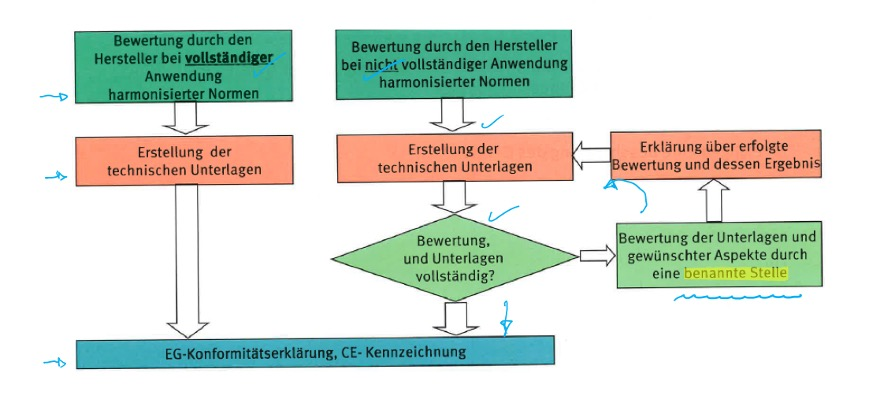
\includegraphics[height=7cm]{src/assets/pictures/lv2_konformitaetsprozess.jpg}
  \caption{Konformitätsbewertungsverfahren}
\end{figure}

\subsection{Was bedeutet das CE Zeichen?}
\begin{itemize}
  \item Das Produkt entspricht \textbf{allen} anzuwendenden Gemeinschaftsvorschriften
  \item Die entsprechenden Konformitätsbewertungsverfahren wurden durchgeführt
  \item Die Mitgliedstaaten dürfen das Inverkehrbringen nicht verhindern (außer das Produkt ist nicht konform)
  \item CE sagt nichts über die Herkunft des Produkts aus
\end{itemize}

\subsection{Dürfen Produkte ohne CE Zeichen in Europa in den Verkehr gebracht werden?}
\textbf{Ja}. Grundsätzlich brauchen Produkte, alle Produkte, die in der EU in Verkehr gebracht werden ein CE Kennzeichen.\p
Die Ausname machen hier ortsfeste Anlagen.

\subsection{Wer haftet wenn Geräte mit CE Zeichen umgebaut werden (müssen) z.B. -Änderung der Sendeantenne eines zertifizierten WLAN Moduls?}
Wenn ein CE gekennzeichnetes Gerät umgebaut und auf den Markt gebracht wird haftet immer derjenige, welcher das Gerät umgebaut hat.

\subsection{Begriffe im Sinne der EMV 2014/30/EU Richtlinie}
\subsubsection{Was ist ein Inverkehrbringer?}
Der Inverkehrbringer ist derjenige, welcher das Produkt auf dem Markt bereitstellt.

\subsubsection{Was ist ein Hersteller?}
Der Hersteller bringt das Gerät in Verkehr. Sie geben Namen, ihren eingetragenen Handlesnamen oder ihre eingetragene Handelsmarke und ihre Postanschrift entweder auf dem Gerät selbst, auf der Verpackung oder in den dem Gerät beigefügten Unterlagen an.

\subsubsection{Was ist ein Gerät?}
Ein fertiger Apparat oder eine als Funktionseinheit in den Handel gebrachte Kombination solcher Apparate, der bzw. die für den Endnutzer bestimmt ist/sind. Ein Gerät kann elektromagnetische Störungen verursachen oder durch sie beeinträchtigt werden.

\subsubsection{Was ist eine Anlage?}
Eine Anlage ist eine besondere Kombination von Geräten unterschiedlicher Art und gegebenenfalls weiteren Einrichtungen, die miteinander verbunden oder installiert werden.\p
Ist die Anlage dazu bestimmt auf Dauer an einem vorbestimmten Ort betrieben zu werden heißt sie \textbf{ortsfest}

\subsubsection{Was ist eine benannte Stelle?}
Staatlich benannte und staatlich überwachte private Prüfstellen.\p
Sie werden von der Kommission in einer Liste im Amtsblatt der EU veröffentlicht.

\subsection{Was passiert mit Geräten die ein CE Zeichen besitzen, nicht den Richtlinien entsprechen und trotzdem am Markt sind?}
Es werden alle zweckdienlichen Maßnamen ergriffen um das Gerät vom Markt zu nehmen, die Inverkehrbringung oder Inbetriebnahme zu untersagen oder den freien Verkehr für diese Gerät einzuschränken (EU-Weite Rückrufaktionen).

\subsection{Was ist eine Konformitätserklärung? Wer muss diese erstellen?}
Eine EU-Konformitätserklärung ist ein \textbf{zwingend notwendiges Dokument}, das entweder Sie als Hersteller oder Ihr bevollmächtigter Vertreter unterschreiben müssen, und mit dem Sie erklären, dass Ihre Produkte den EU-Anforderungen entsprechen. Mit der Unterzeichnung der Konformitätserklärung übernehmen Sie die volle Verantwortung dafür, dass Ihr Produkt dem geltenden EU-Recht entspricht.

\subsection{Wer haftet, bei Verletzung einer CE Erklärung?}
Es haftet derjenige, der die Konformitätserklärung unterzeichnet hat (Hersteller oder seine bevollmächtigten Vertreter).

\pagebreak
\section{Fragen zu Vorlesung 3}

\subsection{Welches Frequenzspektrum hat ein sinusförmiges, welchess ein Pulsförmiges Signal?}\label{sec:lv3:freq_spekt}
\begin{outline}
  \1 \textbf{Sinus:} Einzelner Puls bei der Frequenz des Signals
  \1 \textbf{Puls:} Hoher Puls bei der Frequenz des Signals. Langsam absinkende Pulse bei Vielfachen der Grundfrequenz. (Höherer Puls bei ungeraden Vielfachen)
\end{outline}

\subsection{Welche Signalform generiert die wenigsten Störemissionen?}
Ein Sinussignal, da es nur eine Frequenz besitzt.

\subsection{Wann ist grundsätzlich mit Störemissionen von elektronischen Geräten zu rechnen?}
Störemissionen treten auf wenn sich auf der Platine elektrische- / magnetische (Wechsel-)Felder bilden.

\begin{outline}
  \1 Jedes Gerät \(\rightarrow\) erzeugt elektromagnetische Störung (Elektronenbewegung, Potentialunterschiede)
  \1 Störungsaussendung = leitungsgeführt oder gestrahlt
\end{outline}

\subsection{Welche Maßnahmen können gesetzt werden um breitbandige Störemissionen von Signalen zu reduzieren?}
Glätten der Impulse durch beispielsweise Kapazitäten.

\subsection{Warum entstehen Oberwellenströme bei einem Betrieb von Schaltnetzteilen?}
Durch das Schalten des Transistors. Dadurch entstehen große Spannungssprünge am Knoten nach dem Transistor welche die parasitären Kapazitäten laden bzw. entladen.

\subsection{Erklären Sie das Quellen- Senkenmodell der EMV?}
\begin{outline}
  \1 \textbf{Störquelle:} Ursache von Störungen
  \1 \textbf{Störsenke:} Wird beeinflusst durch Störungen
  \1 \textbf{Koppelpfad:} Störende Verbindung zwischen Quelle und Senke
\end{outline}

\subsection{Welche Arten von Koppelpfaden kennen Sie? Welche Maßnahmen können Sie zur Reduktion der Koppelpfade treffen?}
\begin{outline}
  \1 Galvanische Kopplung
  \1 Nahfeldkopplung
  \1 Einstrahlungsverkopplung
  \1 kapazitive Kopplung
  \1 induktive Kopplung
\end{outline}

\subsection{Erklären Sie eine galvanische Kopplung im Detail. Welche Maßnahmen kennen Sie um eine galvanische Kopplung zu reduzieren}
Entsteht bei einem gemeinsamen Rückleiter (Gemeinsame Masseleitung). Durch Leitungswiderstand entsteht Störspannung, die in die Störsenke gelangt.\p
\textbf{Maßnahmen}
\begin{outline}
  \1 Nur gemeinsamen Massepunkt
\end{outline}


\subsection{Was wird unter Nahfeldkopplung verstanden? Welche dieser Kopplungen kennen Sie?}
Störungen, welche durch niederfrequente elektrische oder magnetische Felder entstehen (bis maximal \(100MHz\)). Oft entstehen diese auf der selben Platine/im selben Gehäuse, wie beispielsweise bei \textbf{kapazitiver} und \textbf{induktiver} Kopplung.


\subsection{Erklären Sie eine kapazitive Kopplung. Wie kommt diese zustanden? Mit welchen Maßnahmen kann Sie reduziert werden}
Verkopplung einzelner Elemente durch parasitäre Kapazitäten (z.B. dadurch, dass Leitungen parallel verlaufen). Tritt nur dann auf, wenn sich das Potential der Elemente unterscheidet.\p
\textbf{Maßnahmen}
\begin{outline}
  \1 Räumliche Trennung
  \1 Reduktion der Leitungslängen
  \1 Einbringen eines Massestreifen zwischen den Leitungen
\end{outline}

\subsection{Erklären Sie eine induktive Kopplung. Wie kommt diese zustande? Welche Maßnahmen kennen Sie um diese zu reduzieren?}
Tritt auf durch (parasitäre) Induktivitäten. Die Induktivitäten einer Stromschleife induziert Strom in eine andere Stromschleife.\p
Die Kopplung wird beschrieben über den \textbf{Koppelfaktor}. Dies ist ein Faktor welcher angibt, wie viel Prozent des Störenden Signals auf die Schaltung wirkt. Die Reduktion des Koppelfaktors reduziert den Einfluss der induktiven Kopplung.\p
\textbf{Maßnahmen}
\begin{outline}
  \1 Räumliche Trennung
  \1 Abstrahlende Fläche, aufnehmende Fläche reduzieren (Leitungen kurz halten, Hin- und Rückleiter parallel zueinander verlegen)
\end{outline}

\subsection{Was ist eine Strahlungskopplung? Wie kommt diese zustande? Welche Maßnahmen kennen Sie um diese zu reduzieren?}
Störung durch einstrahlende höherfrequente Fernfelder (z.B. Elektromagnetische Feldkopplung \textit{LTE, 5G, Radiowellen}).\p
%
\textbf{Maßnahmen}
\begin{outline}
  \1 Verwendung eines geschirmten Gehäuses.
\end{outline}

\subsection{Wie können Störquellen grundsätzlich kategorisiert werden?}
\textbf{Vorkommen}
\begin{outline}
  \1 Dauernde Einwirkung
  \2 Mobilfunk
  \2 Energieversorgung (Stromrichter, Schaltnetzteile) benachbarter Geräte
  \1 Einmalige Einwirkung
  \2 Blitze (Surge)
  \2 Elektrostatische Entladung (ESD)
  \2 Schaltvorgänge (EFT-Burst)
  \2 Spannungseinbrüche
  \2 Radar
\end{outline}
%
\textbf{Auftreten}
\begin{outline}
  \1 Leitungsgeführt
  \2 ESD
  \2 Burst
  \2 Surge

  \1 Eingestrahlt
  \2 Mobilfunk
\end{outline}

\subsection{Wie entstehen Schmalbandstörer?}
Werden von \textbf{periodischen} bzw. getakteten Quellen erzeugt. Schmaler Frequenzbereich
\textbf{Beispiele}
\begin{outline}
  \1 Rundfunkt
  \1 Schaltnetzteile
  \1 Prozessoren
\end{outline}

\subsection{Wie entstehen Breitbandstörer?}
Werden von nicht periodischen bzw. einmaligen \textbf{Störimpulsen} erzeugt. Großer Frequenzbereich bis in \m{GHz} Bereich
\textbf{Beispiele}
\begin{outline}
  \1 ESD
  \1 Blitzentladungen
  \1 Schaltvorgänge
\end{outline}

\subsection{Welche schmalbandigen Störungen kennen Sie?}
\begin{outline}
  \1 Mobilfunk
  \1 Energieversorgung (Stromrichter, Schaltnetzteile) benachbarter Geräte
\end{outline}

\subsection{Welche breitbandigen Störungen kennen Sie?}
\begin{outline}
  \1 Blitze (Surge)
  \1 Elektrostatische Entladung (ESD)
  \1 Schaltvorgänge (EFT-Burst)
  \1 Spannungseinbrüche
  \1 Radar
\end{outline}

\subsection{Was versteht man unter den EMV Prüfungen Surge, Burst, ESD und HF gestrahlt? Welche Störungen werden damit simuliert?}
\begin{outline}
  \1 \textbf{Surge:} Spannungs Impulse (50MHz)
  \1 \textbf{Burst:} Schaltvorgänge (100MHz)
  \1 \textbf{ESD:} Elektrostatische Entladung (100MHz)
  \1 \textbf{HF:} High Frequency
\end{outline}

\subsection{Wie sieht eine beispielhafte Einteilung von Störsenken anhand der Art der Ausfallerscheinung aus? (FSPC = Functional Status Performance Classes)}
\begin{outline}
  \1 Klasse A
    \2 Keine Reaktion auf Störgrößen
    \2 Alle relevanten Parameter befinden sich immer in ihrem übeblichen Toleranzbereich
    \2 Seltene singuläre Ereignisse \m{\rightarrow} z.B. Blitzeinschlag \m{\rightarrow} abrutschen in Klasse B
  \1 Klasse B
    \2 Reaktion des Geräts fällt außerhalb des üblichen Toleranzbereichs
    \2 Nach Abklingen der Störgröße \m{\rightarrow} Rücksprung in Normalzustand
    \2 Nutzen: nicht sicherheitsrelevante Anwendungen \m{\rightarrow} wenn Störgröße dauerhaft vorherrschend \m{\rightarrow} Klasse B nicht zulässig (Funktion dann dauerhaft nicht möglich)
  \1 Klasse C
    \2  Reaktion des Geräts fällt außerhalb des üblichen Toleranzbereichs
    \2 Nach Abklingen der Störgröße \m{\rightarrow} kein Rücksprung in Normalzustand \m{\rightarrow}Benutzereingriff erforderlich
    \2 Gedacht für nicht-sicherheitsrelevante Funktionen \m{\rightarrow} und Phänomene bei welchen ein Hardwarereset selten auftreten
  \1 Klasse D
    \2 System wird nach Störeinwirkung dauerhaft beschädigt \m{\rightarrow} muss von qualifizierter Person repariert werden
    \2 In \textbf{keinem} System zulässig es sei denn \m{\rightarrow} Komfortfunktion (Leselicht im Auto) oder selten auftretende Phänomene
  \1 Klasse FS
    \2 ,,Fail Safe''
    \2 System fällt aufgrund anliegender Störgröße in sicheren Zustand zurück (abschalten, neustarten)
    \2 vergleichbar mit C, jedoch muss Zustand stärker definiert sein \m{\rightarrow} Anforderung höher
    \2 große Maschinen, nur von qualiziertem Personal bedient, darf auch keinen Fall unmotivierte Bewegungen aufgrund von Gewicht oder Motorkraft ausführen
\end{outline}

\pagebreak
\section{Fragen zu Vorlesung 4}

\subsection{Welches Frequenzspektrum hat ein sinusförmiges, welchess ein Pulsförmiges Signal?}
Siehe Fragen~\ref{sec:lv3:freq_spekt}
\begin{itemize}
  \item \textbf{Sinus:} Einzelner Puls bei der Frequenz des Signals
  \item \textbf{Puls:} Hoher Puls bei der Frequenz des Signals. Langsam absinkende Pulse bei Vielfachen der Grundfrequenz. (Höherer Puls bei ungeraden Vielfachen)
\end{itemize}

\subsection{Wann und warum entstehen elektrostatische Aufladungen?}\label{sec:lv4:electrostatic}
Durch große Potentialdifferenzen entstehende Spannungsdurchschläge (durchdringen eines Isolators). Diese Durchschläge bewirken einen kurzen, hohen elektrischen Strom\p
z.B.
\begin{itemize}
  \item Reiben von isolierenden Stoffen
  \item Pos. Ladungsüberschuss auf Glasstab bei Reiben mit Wolle
  \item Auf Textilboden gehende Person -> Aufladung der Person
\end{itemize}

\subsection{Mit welchen Spannungs- und Stromhöhen ist bei ESD zu rechnen?}
\begin{itemize}
  \item Amplituden bis 30kV
  \item Entladeströme 10 bis 100A
\end{itemize}

\subsection{Welche Parameter haben Einfluss auf elektrostatische Aufladungen?}


\subsection{Welches Frequenzspektrum hat ein ESD Puls?}
Breitbandiges Störspektrum

%TODO Foto ESD Entladung Prüfimpuls EN 61000-4-2

\subsection{Welche Anstiegszeit und welche Halbwertszeit hat ein ESD Puls?}
Sehr schnelle Anstiegszeiten Subnanobereich
~ 30 ns Halbwertszeit

\subsection{Wie kann ein ESD Puls in elektronische Schaltungen einkoppeln?}
\begin{itemize}
  \item Galvanisch durch Funkenüberschlag
  \item Induktiv durch di/dt auf geerdete Teile
  \item Kapazitiv durch du/dt auf isolierte metallische Teile
  \item Abstrahlung Magnetfeld durch große di/dt
\end{itemize}

\subsection{Was versteht man unter einen triboelektrischen Effekt?}
Engl.: Triboelectric Charge. Elektrostatische Aufladung durch Berührung/Reibung (Siehe Frage~\ref{sec:lv4:electrostatic}). Verschiebung von Elektronen auf der Metalloberfläche meist durch Berührung und anschließender Trennung. => Ladungstransfer zwischen Körpern mit verschiedenem Potential.

\subsection{Welche Maßnahmen werden zum Schutz von elektrostatischer Entladung gesetzt?}
Abhilfe: ESD-Schutzelemente
\begin{itemize}
  \item ESD Schutzbeschaltung TVS-Dioden
\end{itemize}

\subsection{Was ist der Unterschied zwischen dem HBM und dem MM?}

\subsection{Was ist der Unterschied zwischen Kontakt und Luftentladung? Wann wird welche Entladeart angewandt?}
\textbf{Kontaktentladung}
%TODO Definition
%
\begin{itemize}
  \item gezielt
  \item reproduzierbar
  \item direkt/indirekt
\end{itemize}
%
\textbf{Luftentladung}
%TODO Definition
%
\begin{itemize}
  \item ungezielt
  \item schlecht reproduzierbar
\end{itemize}

\subsection{Von welchen Einflüssen ist die Reproduzierbarkeit der ESD Luftentladung abhängig?}
\begin{itemize}
  \item Ladespannung
  \item Annäherungsgeschwindigkeit
  \item Umgebungsdruck
  \item Luftfeuchtigkeit
\end{itemize}

\subsection{Wie schaut ein ESD Prüfaufbau aus?}
%TODO Foto ESD Entladung Prüfaufbau (direkt)

\subsection{Wann und warum entstehen Burststörungen?}
Burststörungen sind leitungsgeführte Störungen und treten bei schnellen Schaltflanken auf. 

\subsection{Welches Frequenzspektrum hat ein Burstpuls?}
siehe Abbildung \ref{fig:lv4:electro_interferences}
\begin{figure}[ht]
  \centering
  
\includegraphics[height=7cm]{src/assets/pictures/lv4_elektromagnetische_stoerungen.jpg}
  \caption{Elektromagnetische Störungen, Auftreten und Frequenzspektrum}\label{fig:lv4:electro_interferences}
\end{figure}

\subsection{Mit welchen Spannungs- und Stromhöhen ist beim Burststörungen zu rechnen?}

\subsection{Welche Anstiegszeit und welche Halbwertszeit hat ein Burstpuls?}

\subsection{Wie viele Pulse hat ein Burstpaket?}

\subsection{Welche Einkopplungsmöglichkeiten kennt man bei der Burstprüfung?}

\subsection{Wie können Burststörungen in elektronischen Schaltungen reduziert werden?}

\subsection{Wann und warum entstehen Surgestörungen?}
Surgestörungen sind leitungsgeführte Störungen und treten bei Überspannungen durch einen Blitzeinschläge auf. 

\subsection{Welches Frequenzspektrum hat ein Surgepuls?}
siehe Abbildung \ref{fig:lv4:surge_puls}
\begin{figure}[ht]
  \centering
  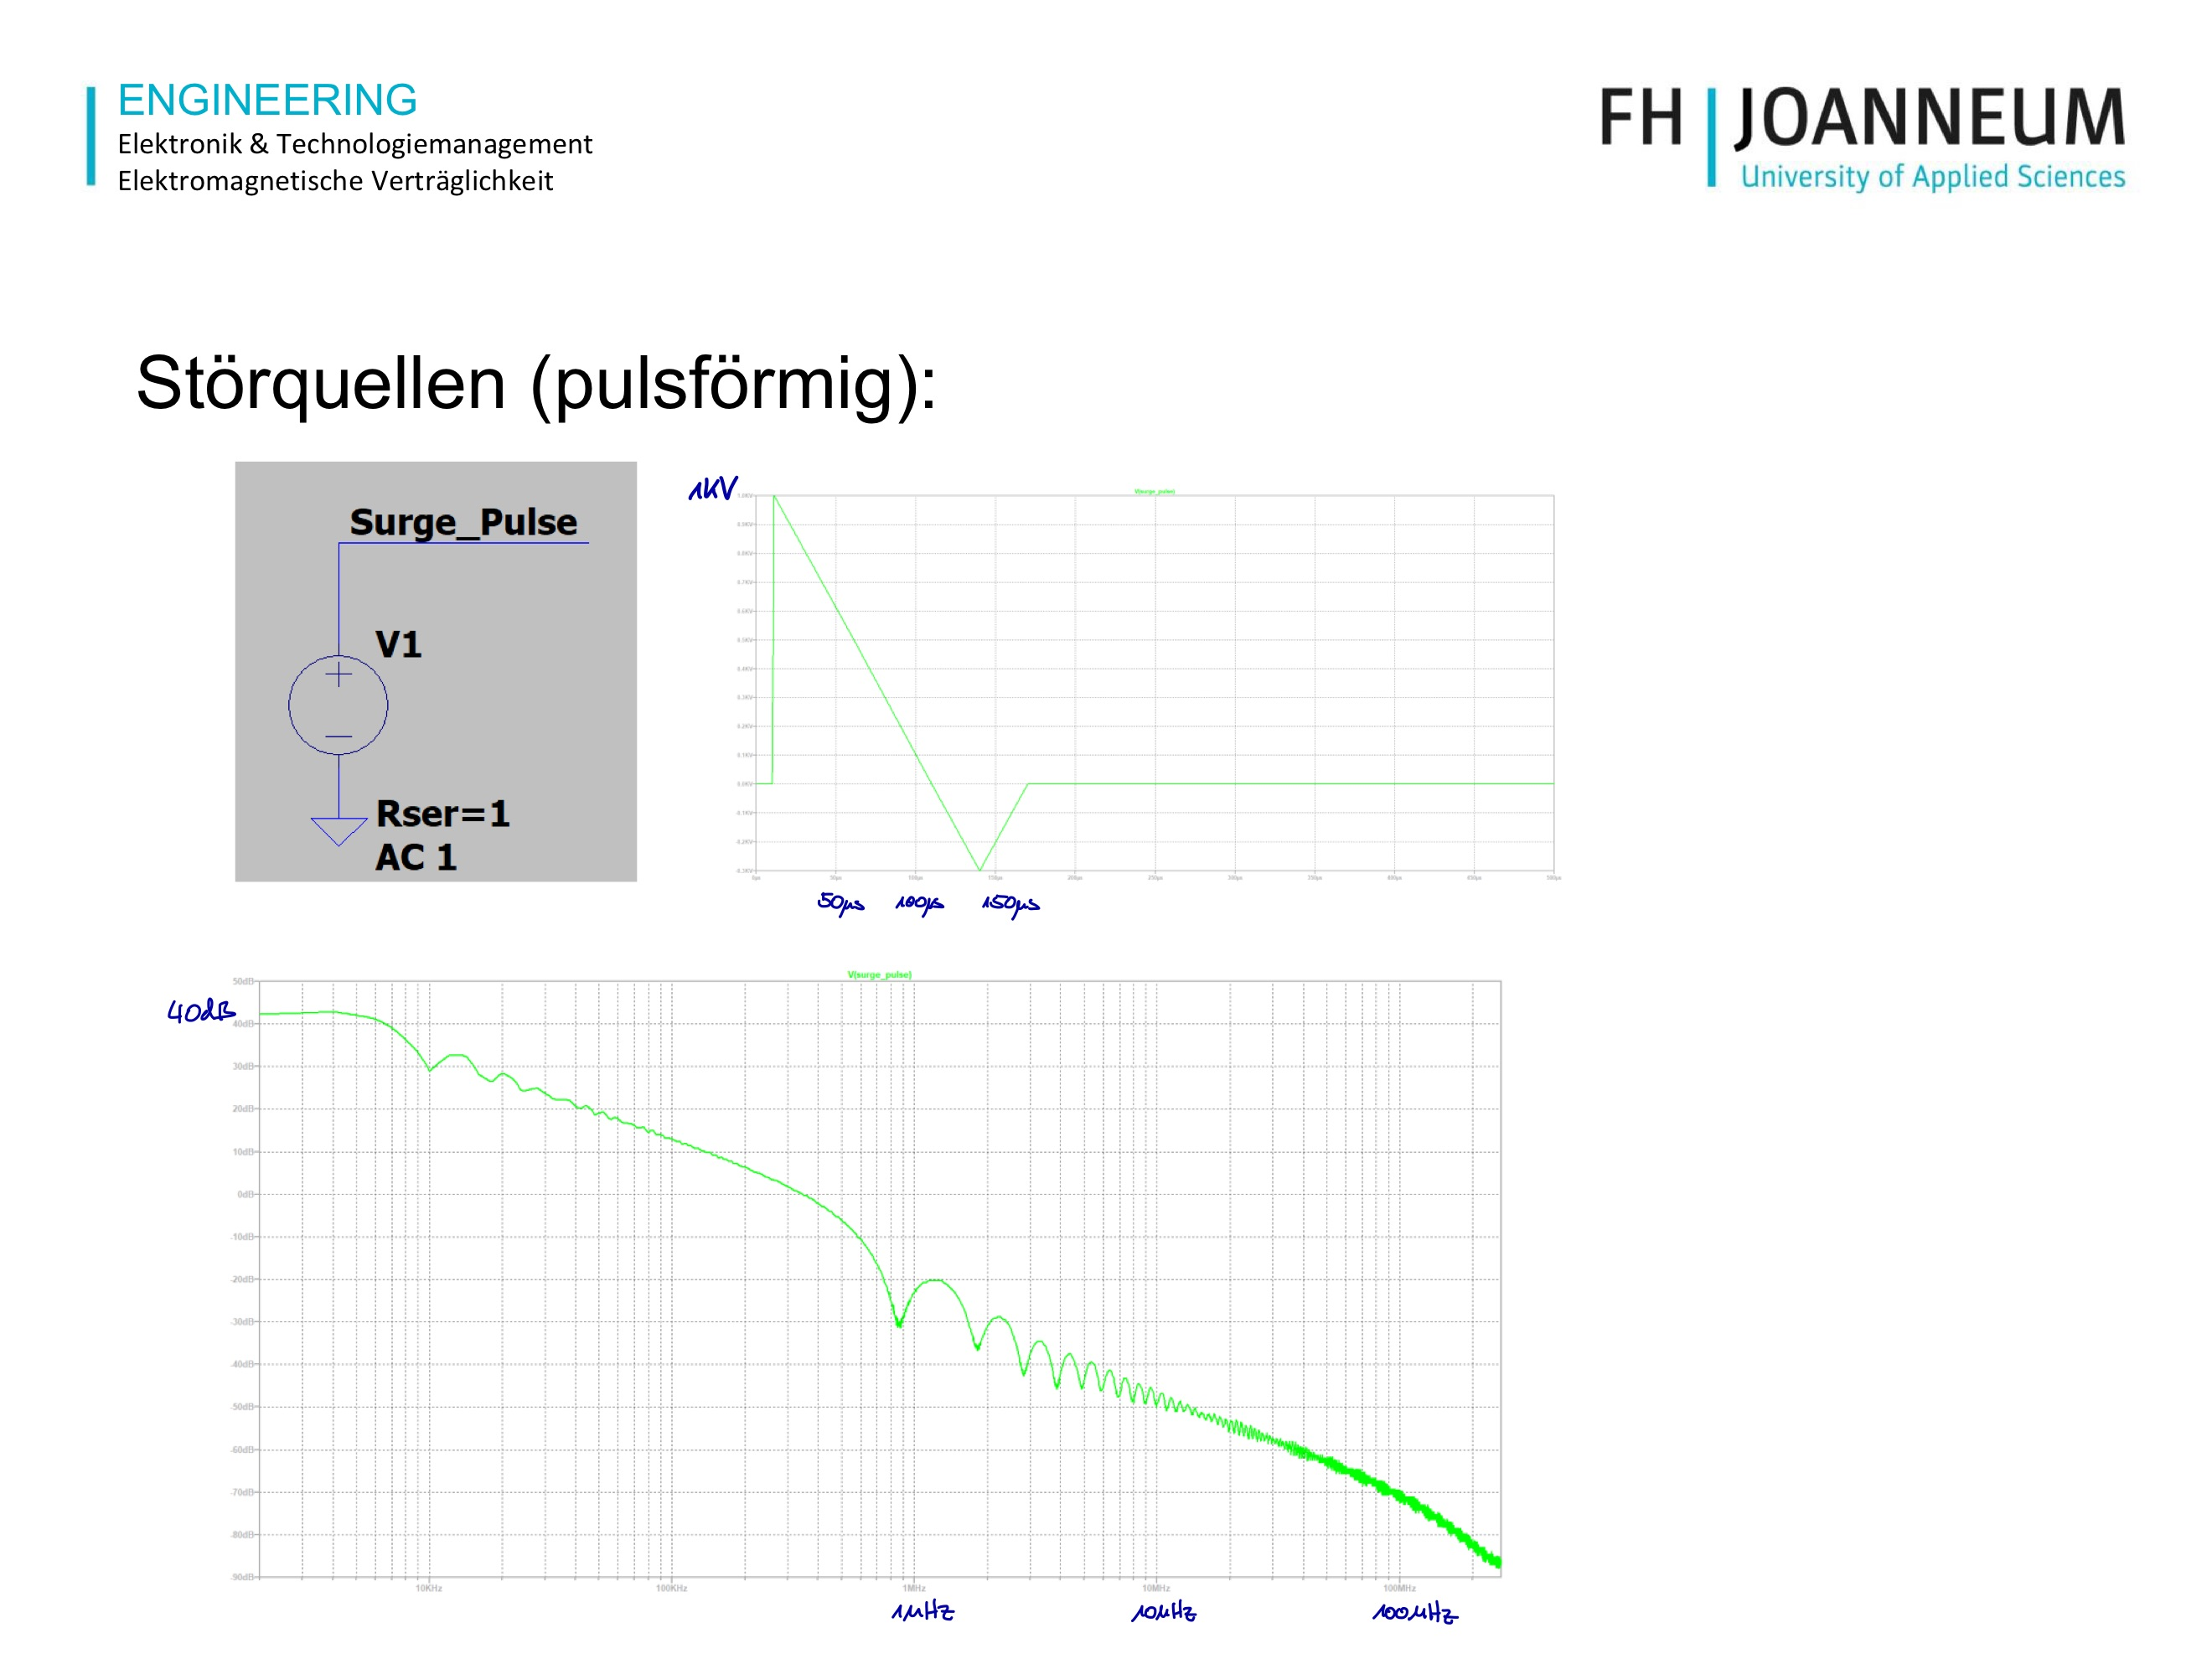
\includegraphics[height=7cm]{src/assets/pictures/lv4_surge_pulse.jpg}
  \caption{Elektromagnetische Störungen, Auftreten und Frequenzspektrum}\label{fig:lv4:surge_puls}
\end{figure}

\subsection{Mit welchen Spannungs- und Stromhöhen ist beim Surge zu rechnen?}
Spannungen bis in den KV-Bereich

\subsection{Wie können elektronische Schaltungen vor Surge geschützt werden?}

\subsection{Auf welchen Leitungen werden Surge- und Burststörungen üblicherweise eingekoppelt?}

\pagebreak


\end{document}

% \enlargethispage{\baselineskip} --> Einige Zeilen trotz seitenumbruch noch auf die vorherige Seite bringen
% \section*{xyz} --> wird nicht im Inhaltsverzeichnis gezeigt